\section{Verwendete Technologien}
Im folgenden Abschnitt werden die Technologien beschrieben, die durch den FreeDesign-Editor genutzt werden und wichtig zum Verständnis der Diplomarbeit sind. 

\subsection{REST-Service}
Die Abkürzung REST steht für 'Representational State Transfer' und beschreibt ein Technologie zu Implementation verteilter Systeme. Mit einem REST-Webservice lassen sich Objekte oder Entitäten zwischen einem Server und einem Client austauschen \autocite[vgl.][S. 105]{Spindler2014}. Zur Kommunikation und dem Dateienaustausch mit den Webservern der Portale in den der FreeDesign-Editor integriert ist, wird eine Vielzahl von REST-Webservices genutzt. Die Webservices werden durch ein eigenes Team innerhalb der IT-Abteilung betreut.  

\subsection{TypeScript}
Für die Implementation des FreeDesign-Editors wird die von Microsoft entwickelte Programmiersprache TypeScript eingesetzt. TypeScript erweitert Javascript um statische Typinformationen und um das Konzept der objektorientierten Programmierung, was sowohl die Lesbarkeit des Quelltextes erhöht, als auch der Fehlervermeidung dient \autocite[vgl.][S. 111]{Zeigermann2014}. Der TypeScript Quelltext wird für die Ausführung im Browser in Javascript übersetzt. Damit ist TypeScript für große Projekte mit mehreren Teammitgliedern, wie dem FreeDesign-Editor, geeigneter als die Implementation in purem Javascript.

\subsection{ReactJS}
Für die Entwicklung einer SPA empfiehlt sich der Einsatz eines Frameworks oder einer Library, welches diesen Ansatz unterstützt. Bereits in der aktuellen Version des Editors kommt hierfür die React-Library, welche von Facebook entwickelt wird, zum Einsatz.
Basierend auf der Dokumentation von Facebook (\cite{Facebook:React}) kann die Funktionalität der React-Library wie folgt zusammengefasst werden.
Eine mit React erstellt Applikation, setzt sich aus einer Vielzahl von React-Komponenten zusammen. Jede React-Komponente besitzt Eigenschaften, die bei dem Instanziieren einer Komponente mit Werten versehen werden, sowie ein internes Statusobjekt. Das zentrale Element einer React-Komponente ist die \emph{render}-Methode, welche basierend auf den Komponenten-Eigenschaften und dem Komponenten-Status einen HTML-Knoten zur Darstellung innerhalb der Applikation rendert. Verändern sich die Eigenschaften oder das Statusobjekt, wird dies von der React-Komponente registriert und die render-Methode wird erneut ausgeführt. Innerhalb des HTML-Knoten, der in der render-Methode einer Komponente beschrieben wird, können weitere React-Komponenten instanziiert und somit in die HTML-Struktur integriert werden.

\subsection{Redux}
Eine Herausforderung für jede SPA ist die Verwaltung applikationsübergreifender Daten sowie das Aktualisieren der Applikation bei Veränderung der Daten.
Einen flexiblen Ansatz bietet die Javascript-Bibliothek \emph{Redux}, welche für die Verwaltung des Status einer SPA entwickelt wurde \autocite[vgl.]{Redux:Introduction}. Durch die Erweiterung \emph{React-Redux} funktioniert Redux besonders gut in Verbindung mit React und erfreut sich großer Beliebtheit unter React-Entwicklern.
Das Redux-Konzept in Verbindung mit React kann, basierend auf der Projekt-Dokumentation (\cite{ReactRedux:QuickStart}), wie folgt umrissen werden. Bei Start der React-Anwendung wird ein zentrales Javascript-Objekt erzeugt, welches sämtliche Statusinformationen der Anwendung enthält. Dieser sogenannte \emph{Store} wird ausschlich durch Redux. Die React-Redux-Bibliothek stellt eine \emph{Provider}-Objekt zur Verfügung, welches Redux, das Store-Objekt und die React-Anwendung miteinander verbindet. Von der selben Bibliothek wird eine \emph{connect}-Funktion bereitgestellt, mit deren Hilfe Properties einer React-Komponente an Daten des Store-Objektes gebunden werden können. Ist es notwendig Informationen im Store zu ändern, geschieht dies durch den Aufruf einer \emph{Action}, was an jeder Stelle der Applikation geschehen kann. Aufgerufen Actions werden von sogenannten Reducern verarbeitet und erzeugen, basierend auf der Action, ein neues Store-Objekt, welches durch Redux aktualisiert wird.
\begin{figure}[H]
\centering
\efbox{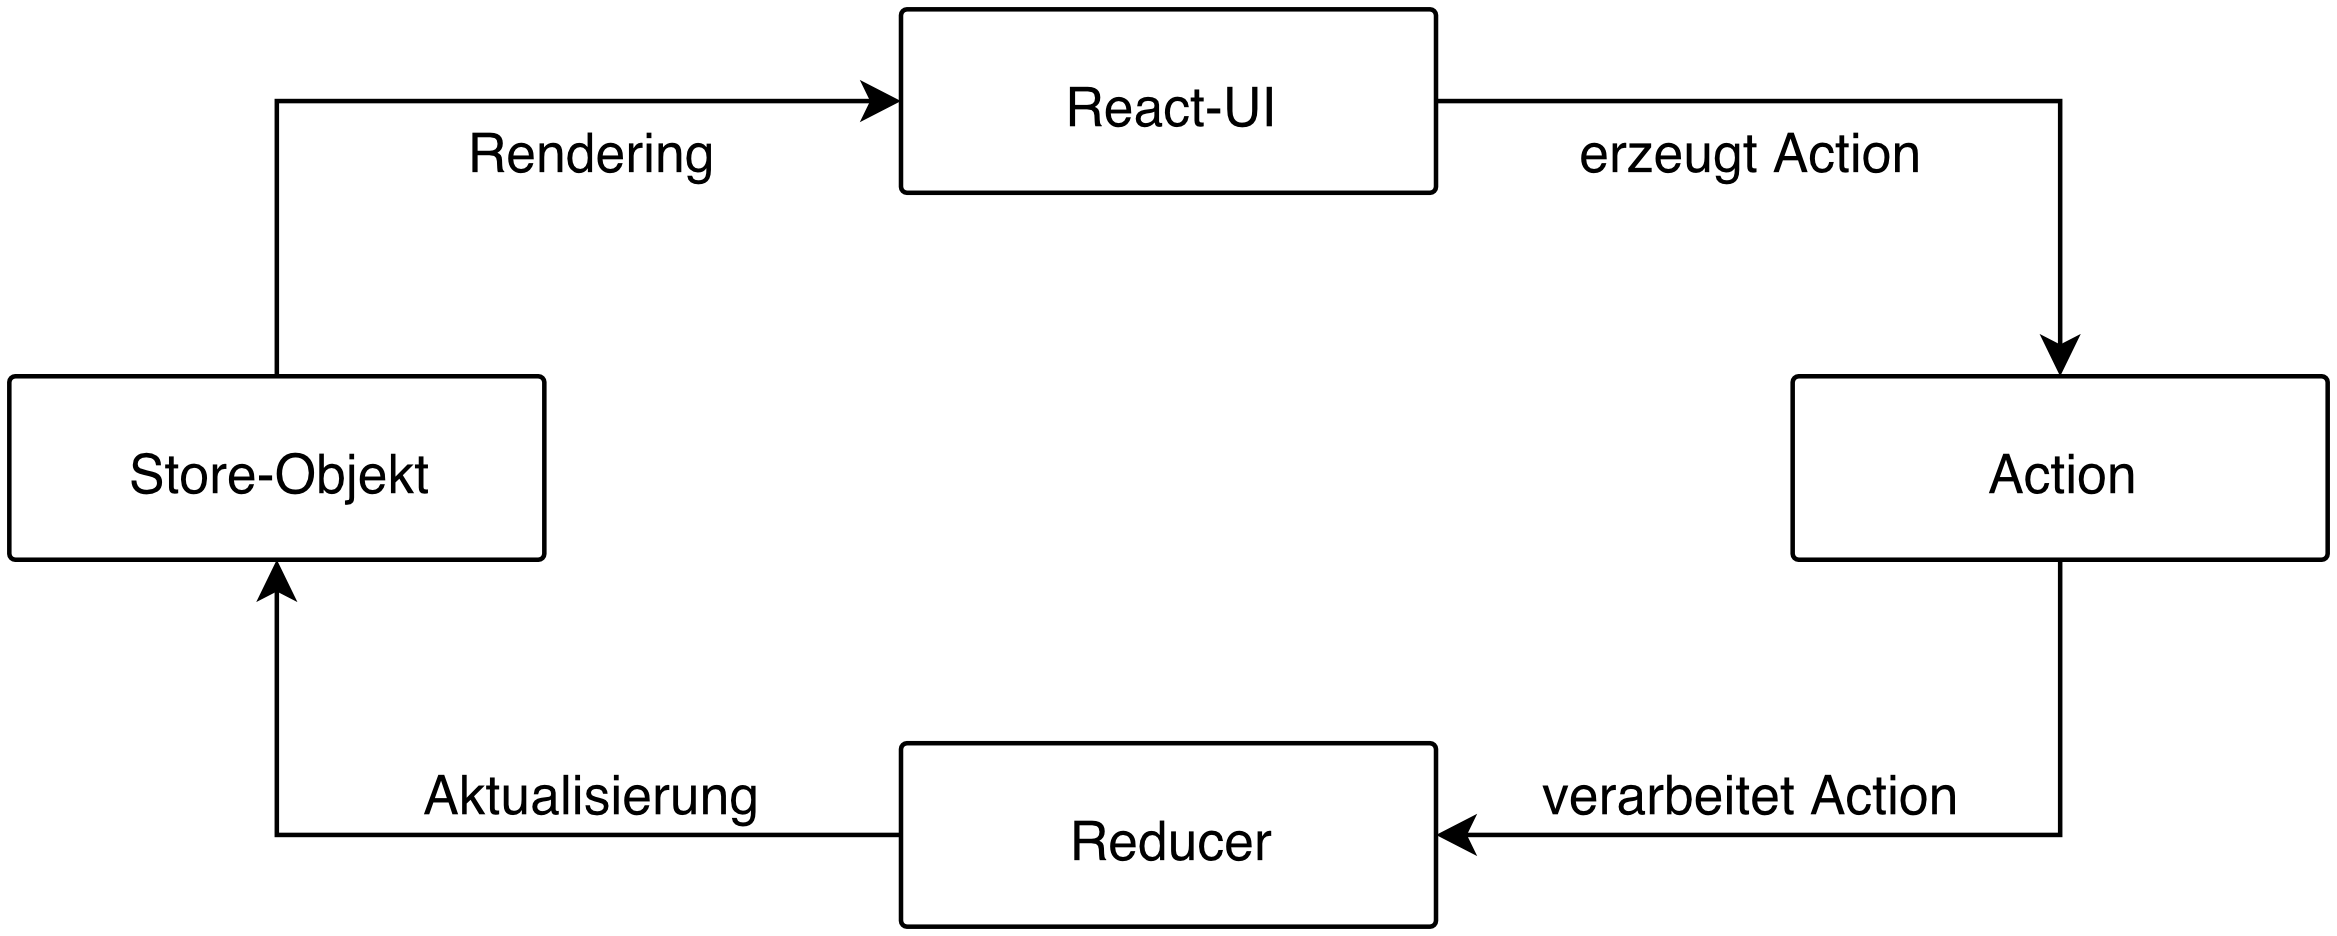
\includegraphics[width=.98\linewidth]{diagrams/ReduxCycle.png}}
\caption[Redux-Zyklus]{der Redux-Zyklus}
\label{figure:ReduxCycle}
\end{figure}
Redux gibt somit einen Kreislauf der Verarbeitung applilaktionsübergreifender Daten vor und bewirkt somit, dass die Darstellung der React-Applikation stets auf dem Store basiert.


\subsection{Jest und Enzyme}
Zum Erstellen von Unit-Tests wurde das Testing-Frameworks Jest eingesetzt, da es ebenfalls durch Facebook entwickelt wird und somit höchstmögliche Kompatibilität mit den React-Komponenten bietet. Weiterhin bietet das Framework als Besonderheit die Erstellung von \emph{Snapshot-Tests}, mit deren Hilfe es sehr einfach ist, die korrekt Struktur von großen Objekten, wie das Rendering von React-Komponenten, sicherzustellen \autocite[vgl.][]{Facebook:JestIntroduction}.
Die Tests werden mit dem Kommandozeilenbefehl \emph{jest} ausgeführt.
Beim Ausführen der Tests analysiert Jest das Projekt und erfasst automatisch Test-Dokumente und führt diese aus. 
Die Erfassung der Test-Dokumente kann jedoch auch eingeschränkt werden, indem bei der Ausführung der Tests ein Teil des Dokumentennamen übergeben wird. Dies beschleunigt den Aufruf einzelner Tests. 
Ergänzt wird der Einsatz des Jest-Frameworks durch die Nutzung der Funktionsbibliothek Enzyme. Enzyme wurde speziell für das Testen von React-Komponenten entwickelt und bietet Funktionalitäten, die das Testen von React-Komponenten erleichtern \autocite[vgl.][]{Enzyme:Introduction}.

\subsection{Das SVG-Format}
Das Format SVG (Scalable Vector Graphics) ist eine XML-basierte Markup-Sprache welche eine Vektorgrafik beschreibt. SVG-Grafiken können *.svg-Dateien gespeichert und innherhalb von HTML-Quelltext platziert werden \autocite[vgl.][]{AboutSVG}. Innerhalb des FreeDesign-Editors wird das SVG-Format für die Produkt- und Designdarstellung, sowie für die Darstellung von Bearbeitungswerkzeugen eingesetzt. 